\documentclass{beamer}

% \documentclass[draft]{beamer}
% \includeonlyframes{wip}

% This file is a solution template for:

% - Giving a talk on some subject.
% - The talk is between 15min and 45min long.
% - Style is ornate.



\mode<presentation>
{
  \usetheme{Pittsburgh}
  % or ...

  % \setbeamercovered{transparent}
  % or whatever (possibly just delete it)
}


\usepackage[dutch]{babel}
\usepackage[utf8]{inputenc}
\usepackage{times}
\usepackage[T1]{fontenc}

\usepackage{mathtools}
\usepackage{tikz}

\usetikzlibrary{arrows,external}
\usepackage{pgfplots}
\pgfplotsset{compat=1.10}
\usepackage[detect-family]{siunitx}
\usepackage[eulergreek]{sansmath}
\sisetup{text-sf=\sansmath}
\usepackage{relsize}


\graphicspath{{figures/}}


\title{Statistische data-analyse 1}
\subtitle{Onzekerheden en de normale verdeling}
\author{David Fokkema}
\institute{
  Practicum natuurkunde \\
  Vrije Universiteit / Universiteit van Amsterdam
}
\date{9 januari 2017}

\subject{Colleges}
% This is only inserted into the PDF information catalog. Can be left
% out.



% If you have a file called "university-logo-filename.xxx", where xxx
% is a graphic format that can be processed by latex or pdflatex,
% resp., then you can add a logo as follows:

% \pgfdeclareimage[height=0.5cm]{university-logo}{university-logo-filename}
% \logo{\pgfuseimage{university-logo}}



% Delete this, if you do not want the table of contents to pop up at
% the beginning of each subsection:
\AtBeginSubsection[]
{
  \begin{frame}<beamer>{Outline}
    \tableofcontents[currentsection,currentsubsection]
  \end{frame}
}


% If you wish to uncover everything in a step-wise fashion, uncomment
% the following command:

%\beamerdefaultoverlayspecification{<+->}


\begin{document}

\begin{frame}
  \titlepage
\end{frame}

\begin{frame}{Outline}
  \tableofcontents
  % You might wish to add the option [pausesections]
\end{frame}


% Since this a solution template for a generic talk, very little can
% be said about how it should be structured. However, the talk length
% of between 15min and 45min and the theme suggest that you stick to
% the following rules:

% - Exactly two or three sections (other than the summary).
% - At *most* three subsections per section.
% - Talk about 30s to 2min per frame. So there should be between about
%   15 and 30 frames, all told.

\section{Inleiding}

\begin{frame}{}
\end{frame}


\section{Onzekerheden}

\begin{frame}{Foutenberekening}
  \begin{itemize}
    \item Vorig jaar: foutenberekening
    \item Onzekerheden uit verschillende bronnen combineren tot totale onzekerheid
    \item Voorbeeld:
    \begin{equation*}
        P = \frac{U^2}{R} \qquad
        \visible<1>
        {\mathrlap{\delta P = \ ?}}
        \visible<2>
        {\mathrlap{\delta P = \sqrt{\left(\frac{\partial P}{\partial U}\delta U\right)^2 + \left(\frac{\partial P}{\partial R}\delta R\right)^2}}}
        \visible<3>
        {\frac{\delta P}{P} = \sqrt{\left(2\frac{\delta U}{U}\right)^2 + \left(\frac{\delta R}{R}\right)^2}}
    \end{equation*}
  \end{itemize}
\end{frame}

\begin{frame}{Onzekerheid verkleinen}
  Hoe verklein je de onzekerheid in een experiment?
  \begin{itemize}
    \item nauwkeuriger meten
    \item<2-> \alert{vaker} meten!
  \end{itemize}
\end{frame}

\begin{frame}{Vaker meten (1)}
  \dots geeft een nauwkeurige schatting van de werkelijke waarde $X$
  \begin{center}
    \begin{tikzpicture}
      \draw[thick] (-5, 0) -- (5, 0);
      \path (0, 30pt) -- (0, -30pt);
      \only<2>{\input{scripts/slide-vaakmeten-gemiddelde-1.out}}
      \only<3>{\input{scripts/slide-vaakmeten-gemiddelde-2.out}}
      \only<4>{\input{scripts/slide-vaakmeten-gemiddelde-3.out}}
      \only<5>{\input{scripts/slide-vaakmeten-gemiddelde-4.out}}
      \only<6>{\input{scripts/slide-vaakmeten-gemiddelde-5.out}}
    \end{tikzpicture}
  \end{center}
  \visible<6>
  {Goede schatter is het gemiddelde $\bar x$:
  \begin{equation*}
    \bar x = \frac{1}{N}\sum_{i=1}^{N} x_i.
  \end{equation*}}
\end{frame}

\begin{frame}{Vaker meten (2)}
  \dots geeft een nauwkeurige schatting van de onzekerheid op \alert{individuele} meting
  \begin{center}
    \begin{tikzpicture}
      \draw[thick] (-5, 0) -- (5, 0);
      \path (0, 35pt) -- (0, -35pt);
      \only<2>{\input{scripts/slide-vaakmeten-stddev-1.out}}
      \only<3>{\input{scripts/slide-vaakmeten-stddev-2.out}}
      \only<4>{\input{scripts/slide-vaakmeten-stddev-3.out}}
      \only<5>{\input{scripts/slide-vaakmeten-stddev-4.out}}
      \only<6->{\input{scripts/slide-vaakmeten-stddev-5.out}}
    \end{tikzpicture}
  \end{center}
  \visible<6>
  {Goede schatter is de standaarddeviatie $\sigma_x$:
  \begin{equation*}
    \sigma_x = \sqrt{\frac{1}{N-1}\sum_{i=1}^{N}(x_i - \bar x)^2}.
  \end{equation*}}
\end{frame}

\begin{frame}{Vaker meten (3)}
  \dots geeft een nauwkeurige schatting van de onzekerheid van de schatting van de werkelijke waarde
  \begin{center}
    \begin{tikzpicture}
      \draw[thick] (-5, 0) -- (5, 0);
      \path (0, 30pt) -- (0, -30pt);
      \only<2>{\input{scripts/slide-vaakmeten-gemiddelde-stdmean-1.out}}
      \only<3>{\input{scripts/slide-vaakmeten-gemiddelde-stdmean-2.out}}
      \only<4>{\input{scripts/slide-vaakmeten-gemiddelde-stdmean-3.out}}
      \only<5>{\input{scripts/slide-vaakmeten-gemiddelde-stdmean-4.out}}
      \only<6>{\input{scripts/slide-vaakmeten-gemiddelde-stdmean-5.out}}
      \only<7>{\input{scripts/slide-vaakmeten-gemiddelde-stdmean-6.out}}
      \only<8>{\input{scripts/slide-vaakmeten-gemiddelde-stdmean-7.out}}
    \end{tikzpicture}
  \end{center}
  \visible<8>
  {Goede schatter is de standaarddeviatie van het gemiddelde $\sigma_{\bar x}$:
  \begin{equation*}
    \sigma_{\bar x} = \frac{\sigma_x}{\sqrt N}.
  \end{equation*}}
\end{frame}

\begin{frame}{Maar\dots}
  \visible<2->{Kan dit gebeuren?} \visible<3->{Ja, helaas\dots}
  \begin{center}
    \begin{tikzpicture}
      \draw[thick] (-5, 0) -- (5, 0);
      \path (0, 35pt) -- (0, -20pt);
      \input{scripts/slide-vaakmeten-gemiddelde-5.out}
      \only<2->{\draw[red] (-4, 10pt) -- +(0, -20pt) node[below] {$X$};}
      \only<3->{\draw[<->,red] (-4, 15pt) -- node[above] {systematische fout} (1.0238117778, 15pt);}
    \end{tikzpicture}
  \end{center}
  \visible<4>
  {Goede schatter voor de totale fout:
  \begin{equation*}
    \delta x_\mathrm{tot} = \sqrt{(\delta x_\mathrm{ran})^2 + (\delta x_\mathrm{sys})^2}.
  \end{equation*}}
\end{frame}

\begin{frame}{Samenvattend}
  \begin{itemize}
    \item schatter werkelijke waarde:
    \begin{equation*}
      \bar x = \frac{1}{N}\sum_{i=1}^{N} x_i. \qquad \text{(gemiddelde)}
    \end{equation*}
    \item schatter onzekerheid van individuele meting:
    \begin{equation*}
      \sigma_x = \sqrt{\frac{1}{N-1}\sum_{i=1}^{N}(x_i - \bar x)^2}. \qquad \text{(standaarddeviatie)}
    \end{equation*}
    \item schatter onzekerheid op schatter werkelijke waarde:
    \begin{equation*}
      \sigma_{\bar x} = \frac{\sigma_x}{\sqrt N}. \qquad \text{(stddev van het gemiddelde)}
    \end{equation*}
  \end{itemize}
\end{frame}


\section{De normale verdeling}

\begin{frame}{Representatie van veel metingen}
  Meetwaardes:
  \begin{center}
    \input{scripts/slide-representaties-numbers.out}
  \end{center}
\end{frame}

\begin{frame}{Representatie van veel metingen}
  Getallenlijn:
  \begin{center}
    \begin{tikzpicture}
      \draw[thick] (-5, 0) -- (5, 0);
      \path (0, 35pt) -- (0, -20pt);
      \input{scripts/slide-representaties-getallenlijn.out}
    \end{tikzpicture}
  \end{center}
\end{frame}

\begin{frame}{Representatie van veel metingen}
  Histogram:
  \begin{center}
    \input{scripts/slide-representaties-histogram-1}
  \end{center}
\end{frame}

\begin{frame}{Limietverdeling}
  \begin{center}
    \only<1>{\input{scripts/slide-representaties-histogram-N-1}}

    \only<2>{\input{scripts/slide-representaties-histogram-N-2}}

    \only<3>{\input{scripts/slide-representaties-histogram-N-3}}

    \only<4>{\input{scripts/slide-representaties-histogram-N-4}}

    \only<5>{\input{scripts/slide-representaties-histogram-N-5}}

  \end{center}
\end{frame}

\begin{frame}{Normale verdeling}
  \begin{center}
    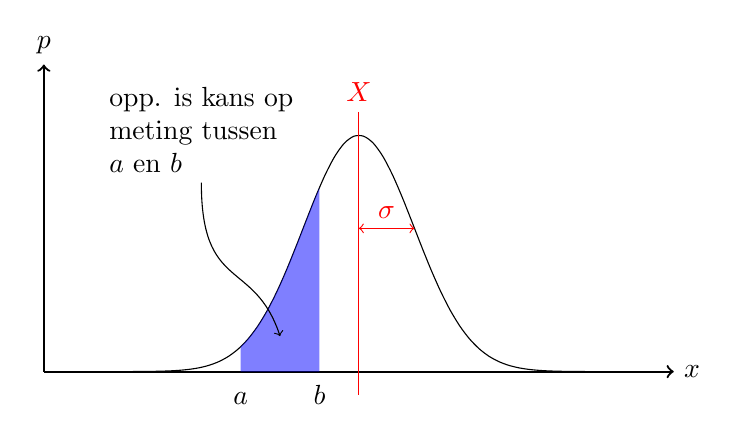
\begin{tikzpicture}[yscale=3]
      % axis
      \draw[thick,->] (-4, 0) -- (4, 0) node[right] {$x$};
      \draw[thick,->] (-4, 0) -- +(0, 1.3) node[above] {$p$};
      % function
      \draw plot[domain=-3:3,samples=50,smooth] (\x, {exp(-(\x*\x))});
      % labels
      \visible<2->{\draw[red] (0, 1.1) node[above] {$X$} -- (0, -.1);}
      \draw<3->[<->,red] (0, 0.6065) -- node[above] {$\sigma$} (0.707, 0.6065);
      % region
      \visible<4->{
        \fill[blue, opacity=.5] (-1.5, 0) -- plot[domain=-1.5:-.5,samples=50,smooth] (\x, {exp(-(\x*\x))}) -- (-.5, 0);
        \node[anchor=base] at (-1.5, -4pt) {$a$};
        \node[anchor=base] at (-.5, -4pt) {$b$};
        \draw[align=left,->] (-2, .8) node[above] {opp. is kans op\\ meting tussen\\ $a$ en $b$} to[out=-90] (-1, .15);
      }
    \end{tikzpicture}
  \end{center}
  \begin{equation*}
    G_{X,\sigma}(x) = \frac{1}{\sigma\sqrt{2\pi}}\,e^{-(x - X)^2 / 2\sigma^2}
  \end{equation*}
\end{frame}

\begin{frame}{Normale verdeling}
  \begin{center}
    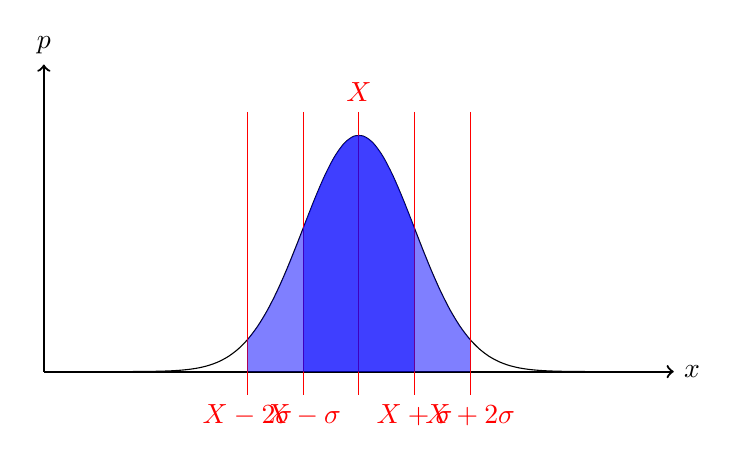
\begin{tikzpicture}[yscale=3]
      % axis
      \draw[thick,->] (-4, 0) -- (4, 0) node[right] {$x$};
      \draw[thick,->] (-4, 0) -- +(0, 1.3) node[above] {$p$};
      % function
      \draw plot[domain=-3:3,samples=50,smooth] (\x, {exp(-(\x*\x))});
      % labels
      \draw[red] (0, 1.1) node[above] {$X$} -- (0, -.1);
      \draw<1>[red] (0.707, 1.1) -- (0.707, -.1) node[below] {$X + \sigma$};
      \draw<1>[red] (-0.707, 1.1) -- (-0.707, -.1) node[below] {$X - \sigma$};
      \draw<2>[red] (1.414, 1.1) -- (1.414, -.1) node[below] {$X + 2\sigma$};
      \draw<2>[red] (-1.414, 1.1) -- (-1.414, -.1) node[below] {$X - 2\sigma$};
      % region
      \fill<1>[blue, opacity=.5] (-0.707, 0) -- plot[domain=-0.707:0.707,samples=30,smooth] (\x, {exp(-(\x*\x))}) -- (0.707, 0);
      \fill<2>[blue, opacity=.5] (-1.414, 0) -- plot[domain=-1.414:1.414,samples=30,smooth] (\x, {exp(-(\x*\x))}) -- (1.414, 0);
    \end{tikzpicture}
  \end{center}
  \only<1>{Kans van \SI{68}{\percent} dat meting binnen \SI{1}{\sigma} van de werkelijke waarde valt.}
  \only<2>{Kans van \SI{95}{\percent} dat meting binnen \SI{2}{\sigma} van de werkelijke waarde valt.}
\end{frame}

\begin{frame}{Error function}
  \begin{center}
    % \usepackage{tikz}
% \usetikzlibrary{arrows,external}
% \usepackage{pgfplots}
% \pgfplotsset{compat=1.10}
% \usepackage[detect-family]{siunitx}
% \usepackage[eulergreek]{sansmath}
% \sisetup{text-sf=\sansmath}
% \usepackage{relsize}
%
    \tikzsetnextfilename{externalized-slide-errorfunction}
\pgfkeysifdefined{/artist/width}
    {\pgfkeysgetvalue{/artist/width}{\defaultwidth}}
    {\def\defaultwidth{ .67\linewidth }}
%
%
\begin{sansmath}
\begin{tikzpicture}[
        font=\sffamily,
        every pin/.style={inner sep=2pt, font={\sffamily\smaller}},
        every label/.style={inner sep=2pt, font={\sffamily\smaller}},
        every pin edge/.style={<-, >=stealth', shorten <=2pt},
        pin distance=2.5ex,
    ]
    \begin{axis}[
            axis background/.style={  },
            xmode=normal,
            ymode=normal,
            width=\defaultwidth,
            scale only axis,
            axis equal=false,
            %
            title={  },
            %
            xlabel={ grenzen [$\sigma$] },
            ylabel={ kans waarde binnen grenzen [\%] },
            %
            xmin={ 0 },
            xmax={ 4 },
            ymin={ 0 },
            ymax={ 1 },
            %
            xtick={ 0, 0.674, 1.0, 2.0, 3.0, 4.0 },
            ytick={ 0, 0.5, 0.68, 0.95, 1.0 },
            xticklabel style={  },
            yticklabel style={  },
            %
            tick align=outside,
            max space between ticks=40,
            every tick/.style={},
            axis on top,
            point meta min={  },
            point meta max={  },
            colormap={coolwarm}{
                rgb255=( 59, 76,192)
                rgb255=( 98,130,234)
                rgb255=(141,176,254)
                rgb255=(184,208,249)
                rgb255=(221,221,221)
                rgb255=(245,196,173)
                rgb255=(244,154,123)
                rgb255=(222, 96, 77)
                rgb255=(180,  4, 38)},
            colormap={whiteblack}{gray=(1) gray=(0)},
            colormap={blackwhite}{gray=(0) gray=(1)},
        ]


    \draw[gray] (axis cs:0, .5) -| (axis cs:.674, 0);
    \draw[gray] (axis cs:0, .68) -| (axis cs:1, 0);
    \draw[gray] (axis cs:0, .954) -| (axis cs:2, 0);


    % Draw series plot
    \addplot[no markers,solid] coordinates {
            (0.0, 0.0)
            (0.08, 0.063762744028)
            (0.16, 0.127118925783)
            (0.24, 0.189669743396)
            (0.32, 0.251031669447)
            (0.4, 0.310843483221)
            (0.48, 0.368772606968)
            (0.56, 0.424520562302)
            (0.64, 0.477827400614)
            (0.72, 0.528475004441)
            (0.8, 0.576289202833)
            (0.88, 0.621140690447)
            (0.96, 0.662944785066)
            (1.04, 0.701660099338)
            (1.12, 0.737286237915)
            (1.2, 0.769860659557)
            (1.28, 0.799454864091)
            (1.36, 0.826170076106)
            (1.44, 0.850132600931)
            (1.52, 0.871489024362)
            (1.6, 0.890401416601)
            (1.68, 0.907042684273)
            (1.76, 0.921592193425)
            (1.84, 0.934231762682)
            (1.92, 0.945142100592)
            (2.0, 0.954499736104)
            (2.08, 0.96247446713)
            (2.16, 0.969227330432)
            (2.24, 0.974909077128)
            (2.32, 0.979659122663)
            (2.4, 0.983604928151)
            (2.48, 0.986861761729)
            (2.56, 0.989532783673)
            (2.64, 0.991709397278)
            (2.72, 0.993471808368)
            (2.8, 0.994889739339)
            (2.88, 0.99602324829)
            (2.96, 0.996923609577)
            (3.04, 0.997634218514)
            (3.12, 0.9981914896)
            (3.2, 0.998625724124)
            (3.28, 0.998961929134)
            (3.36, 0.999220575275)
            (3.44, 0.999418285813)
            (3.52, 0.999568453201)
            (3.6, 0.99968178282)
            (3.68, 0.999766766046)
            (3.76, 0.999830086643)
            (3.84, 0.99987696569)
            (3.92, 0.999911451031)
            (4.0, 0.999936657516)
    };



    \end{axis}
\end{tikzpicture}
\end{sansmath}

  \end{center}
\end{frame}

\begin{frame}{Weergeven van resultaat}
  Geef het eindresultaat van je metingen als volgt:

  \vspace{1em}

  schatter werkelijke waarde $\pm$ schatting fout op die waarde
  \uncover<2->{
  \begin{equation*}
    \bar x \pm \sigma_{\bar x}
  \end{equation*}}%
  \uncover<3->{(Slordig) \SI{68}{\percent} kans dat de werkelijke waarde binnen de grenzen valt}
\end{frame}


\section*{Samenvatting}

\begin{frame}{Samenvatting}

  Vandaag behandeld:
  % Keep the summary *very short*.
  \begin{itemize}
  \item
    Het gemiddelde, de standaarddeviatie en de standaarddeviatie van het gemiddelde
  \item
    Meetwaardes onder invloed van veel kleine toevallige fouten zijn \alert{normaal verdeeld}
  \item
    Het \alert{gemiddelde} en de \alert{standaarddeviatie van het gemiddelde} zijn de beste schatters voor de werkelijke waarde en de onzekerheid (\SI{68}{\percent})
  \end{itemize}

\end{frame}


\end{document}
